
Las \textbf{RNA} son una estructura compuesta de un número de unidades interconectadas (neuronas artificiales), cada unidad posee una característica entrada/salida e implementa una computación local o función, la salida de cualquier unidad esta determinada, su interconexión con otras unidades, y posiblemente de sus unidades internas. La red desarrolla usualmente una funcionalidad por lo general a través de una o mas formas, por lo tanto es un arreglo masivo de elementos de procesamiento simple llamados neuronas, los cuales poseen un alto grado de interconectividad entre sus elementos, en los que la información puede fluir en cascada potenciando su capacidad para aproximar funciones, clasificar patrones y aumenta su inmunidad frente al ruido. 

El modelo genérico de neurona artificial se puede ver en la Fig. \ref{generico}, en este se puede visualizar el funcionamiento simple de una neurona en forma de un procesador elemental, que a partir de un vector de entrada procedente del exterior o de otras neuronas, proporcionando una única respuesta o salida.

\begin{figure}[!t]
\centering
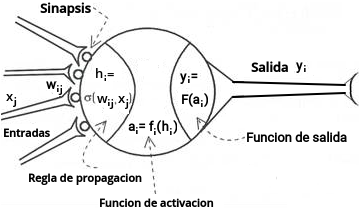
\includegraphics[width=.7\textwidth]{Cap3/imagenes/generico.png}
\caption[Modelo genérico de una neurona artificial.]{Modelo genérico de una neurona artificial.\footnote{Página de origen: \href{https://grupo.us.es/gtocoma/pid/pid10/RedesNeuronales.htm}{https://\-gru\-po.\-us.\-es/\-gto\-coma/\-pid/\-pid10/\-Re\-des\-Neu\-ro\-na\-les.\-htm}}}
\label{generico}
\end{figure}

Los elementos que constituyen neurona genérica se pueden observar en la Fig. \ref{generico}, siendo $x_j(t)$ las variables de entrada y salida, los pesos sinápticos $w_{ij}$ representan la intensidad de interacción entre cada neurona presináptica $j$ y la neurona postsináptica $i$. Las reglas de propagación $\sigma(w_{ij}, x_j(t))$ proporcionan el valor del potencial postsináptico, $h_i(t)$, de la neurona $i$ en función de sus pesos $w_{ij}$ y entradas $x_i(t)$, la usada en esta investigación es $h_i (t) = \sum_j w_{ij} x_j$. La función de activación o de transferencia $a_i(t) = f_i(h_i(t))$ proporciona el estado de activación de la neurona en función del estado anterior y del valor postsináptico. Además, $y_i(t) = F(h_i(t))$ representa la simultáneamente la salida de la neurona y su estado de activación. 

Para la optimización de la redes implementadas es resultado de la utilización del algoritmo de optimización de Adam, siendo este una extensión del descenso de gradiente estocástico\citep{adam}. Dado que es un conjunto de nodos interconectados, estás realizan al menos una de las siguientes funciones: aprendizaje, memorización, generalización o abstracción de características a partir de un conjunto de datos, adaptación y tolerancia a fallos, este será utilizado para identificar di-muones característicos del decaimiento \textbf{Dark-}\SUSY (ver Fig. \ref{fig:sketch_darksector}) y como método alternativo regresión al mostrado en la sección \ref{Cap_regresion}.

\subsection{Identificando y reconstruyendo el fotón oscuro}\label{identificador_sec}

Es de gran interés en esta investigación la creación de una metodología de identificación de di-muones, que pueda discernir entre los muones provenientes de la señal \MSSM\textbf{D}, emparejarlos y reconstruir correctamente el fotón oscuro del cual teóricamente se espera que hayan decaído según el diagrama de la Fig. \ref{fig:sketch_darksector}b. Esta herramienta de identificación, puede crearse, haciendo uso de las redes artificiales neuronales, ya que ella puede ser una herramienta robusta en el reconocimiento de patrones y objetos.     .

\begin{figure}[!h]
\centering
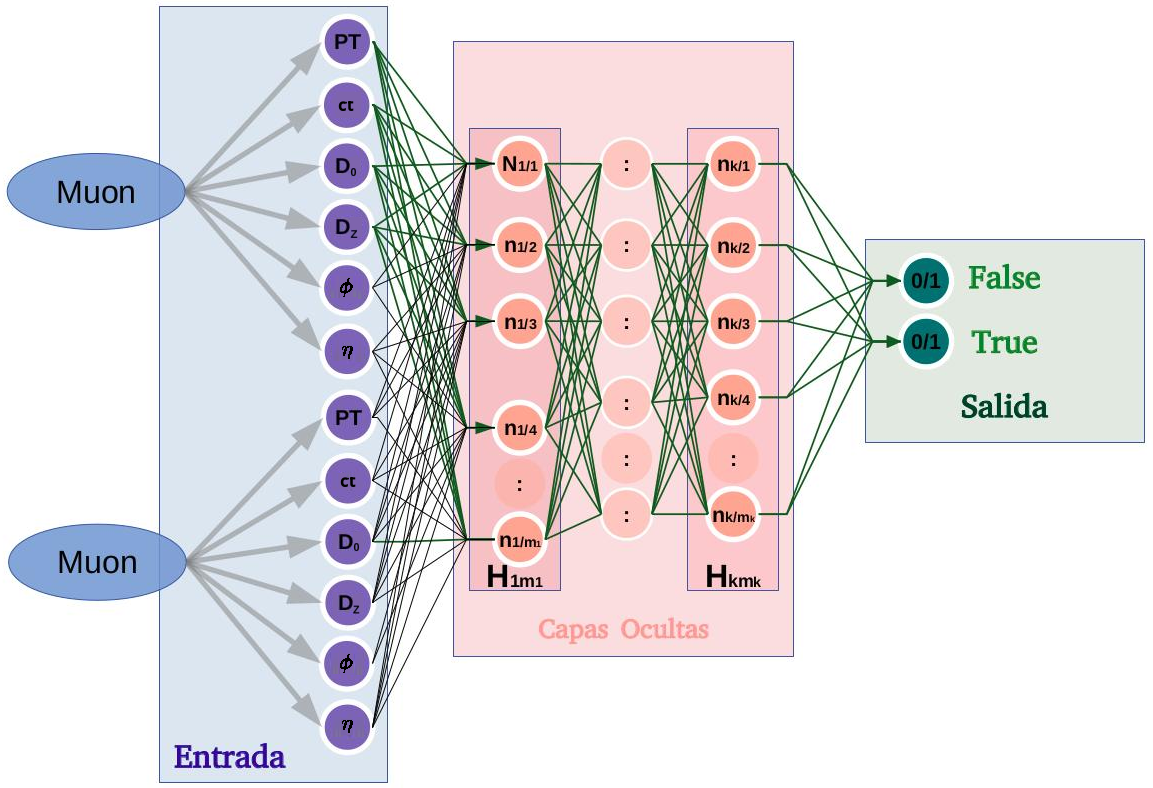
\includegraphics[width=.9\textwidth]{Cap4/imagenes/IDENTIFICADOR.png}
\caption{Diagrama de la estructura de la red neuronal dedicada a la identificación de di-muones provenientes del fotón oscuro $\gamma_D$.}
\label{identificador}
\end{figure}

Se crea una red artificial que dadas las propiedades de los di-muones, pueda informar si esta selección proviene o no de un fotón oscuro del decaimiento \textbf{Dark-}\SUSY%\MSSM\textbf{D} 
~(ver Fig. \ref{identificador}). La creación de datos de entrada que serán usados para entrenamiento es resultado de generar todos los posibles emparejamientos por eventos dentro de la clase $\textsf{GenParticle}$ en el árbol de los archivos $\textsf{*.root}$ y generar una salida binaria correspondiente a las partículas que declara la correcta o incorrecta selección de muones según sus propiedades $\textsf{x}_{ij}$, también se incluyen en los datos variaciones en los parámetros de generación $\vec{\alpha}$. Los datos que corresponden a las entrada de la red $\mathtt{x}_{ij}$ y las salidas $\mathtt{y}_i$ fueron obtenidos de las muestras simuladas con variación en los parámetros de generación $\vec{\alpha}$. 


Este problema, es equivalente al perceptrón simple, siendo una de las caracterizaciones más básicas en el área de redes neuronales artificiales. Para implementar este identificador se hace uso de las paqueterías o herramientas de \textsfSmall{keras} programando en el entorno de \textsfSmall{python}. Se hace necesario funciones de activación específicas que incluyan las entradas $\textsf{x}_{ij}$ y las salidas $\textsf{x}_i$, las primeras ante la necesidad de reacondicionamiento ante la gran diferencia de rango de los dominios de las variables $\textsf{x}_{ij}$, las salidas deben ser dadas en forma de probabilidades de tal manera que el sumatoria de las salidas sea normalizada y de esta manera poder imponer criterios de binarización. Dado lo cual, se utilizó la tangente hiperbólica $\textsf{Tanh}$ para la que conexión entre las capas de entrada con las primeras capas ocultas $x_{ij} \longrightarrow m_1$:
\begin{equation}
f(x)=\dfrac{2}{1+e^{-2x}}-1
\end{equation}
Para las capas de salida $m_k \longrightarrow y_i$ se utiliza la función $\textsf{Softmax}$:
\begin{equation}
f(x)_j = \dfrac{e^{Z_j}}{\sum_{k=1}^{K}e^{Z_k}}
\end{equation}
La función de activación utilizada para relacionar todas las capas ocultas es una lineal rectificada \textsfSmall{ReLU} \footnote{Las funciones https://www.diegocalvo.es/funcion-de-activacion-redes-neuronales/} dada por:
\begin{equation}\label{relu}
\mathtt{f(x)=\max (0,x)} ~ = ~ \Bigg\{\begin{matrix}
0 & \mathtt{para }~ x<0\\
x & \mathtt{para }~ x\geq 0\\
\end{matrix} 
\end{equation}

Para poder caracterizar la precisión del modelo clasificatorio implementado, la relación entre el número de predicciones correctas y el número total de muestras de entrada nos permitirá conocer la eficiencia del clasificador:
\begin{equation}\label{acc}
\textsf{acc} =  \dfrac{\textsf{Número de predicciones correctas}}{\textsf{Numero total de predicciones}}
\end{equation}

Se implementa una caracterización para diferentes combinación de parámetros $\textsf{x}_{j}$ como entradas, manteniendo constante la cantidad de épocas y donde se consideraron $\textsf{k}=1,\ldots,6$ capas ocultas con una cantidad de neuronas dadas por $\textsf{m}_k = 128, 64, 32, 16, 8, 4$, los resultados se muestran en la Tabla \ref{ajuste1}.

\begin{table}[!h]
\footnotesize
\centering
\begin{tabular}{|cccccc|c||cccccc|c|}
\toprule
\multicolumn{6}{|c|}{$\textsf{x}_j$ consideradas} &  &
\multicolumn{6}{|c|}{$\textsf{x}_j$ consideradas} &  \\
\midrule
%$PT$ & $T$ & $D0$ & $DZ$ & $Phi$ & $Eta$ & \textsf{accy} &
%$PT$ & $T$ & $D0$ & $DZ$ & $Phi$ & $Eta$ & \textsf{accy} \\
%\midrule
$P_T$ & $\phi$ & $\eta$ & $c\tau$ & $D_0$ & $D_Z$  & \textsf{accy} &
$P_T$ & $\phi$ & $\eta$ & $c\tau$ & $D_0$ & $D_Z$  & \textsf{accy} \\
\midrule
SI & NO & NO & NO & NO & NO & $0.61 \pm 0.16$ & 
NO & NO & NO & SI & NO & NO & $0.63 \pm 0.05$\\
NO & SI & NO & NO & NO & NO & $0.82 \pm 0.04$ & 
NO & NO & NO & NO & SI & NO & $0.62 \pm 0.07$\\  
NO & NO & SI & NO & NO & NO & $0.90 \pm 0.03$ & 
NO & NO & NO & NO & NO & SI & $0.64 \pm 0.04$\\
\bottomrule
SI & SI & SI & NO & NO & NO & $0.93 \pm 0.01$ &
NO & SI & SI & NO & NO & NO & $0.95 \pm 0.02$\\
\bottomrule 
\end{tabular}%}
\caption{Capacidad del identificador fotónico con variaciones en los parámetros de entrada.}
\label{ajuste1}
\end{table}

\begin{figure}[!h]
\centering
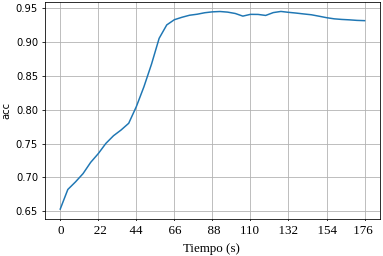
\includegraphics[width=.5\textwidth]{Cap4/imagenes/acc.png}
\caption{Variación de la precisión del identificador durante el proceso de entrenamiento con el tiempo para una configuración de entrada dada por los $x_i = (\eta, \phi)$.}
\label{identificador0}
\end{figure}

De la interpretación de los resultados de la Tabla \ref{ajuste1} se concluye que las propiedades $P_T, ~ c\tau, ~ D_0, ~D_Z$ no son determinantes en la identificación de los di-muones, el origen de estos resultados puede estar dado por la inclusión de casos para tiempos teóricos de vida 0, cuestión no valorada en esta investigación. Por el contrario las propiedades $\eta$ y $\phi$ muestran potencial válidado en el \textsf{accy} $\gtrsim$ 0.80 razón por la cual son elegidos para formar parte de las entradas del entrenamiento final. 

De concluyó que la creación de una herramienta identificadora de di-muones con las entradas consideradas para $\textsf{x}_j=(\eta,\phi)$ es la más adecuada encontrada, con un \textsf{accy} $= 0.95 \pm 0.02$ (ver Fig. \ref{identificador0}) se presenta con bajos errores que la hacen una herramienta suficientemente robusta para una investigación en la que se esperan resultados fiables. La implementación de un entrenamiento de está índole disminuiría el tiempo de cómputo, manteniendo una alta fiabilidad en los resultados obtenidos.


\subsection{Regresión de datos}

Los modelos de redes neuronales pueden ser considerados como nuevos paradigmas para el análisis estadístico de regresión lineal. Una de las razones del uso de las redes neuronales es que no necesitan el cumplimiento de supuestos teóricos como en los modelos estadísticos clásicos. El modelo del Perceptrón multicapa es equivalente a un modelo de regresión lineal, debido a la similitud de la variable de salida que se relaciona aplicando la función de activación sobre una combinación lineal de pesos con las variables de entrada. 

Para la implementación de la regresión mediante \textbf{RNA}, se hizo uso de una estructura como la mostrada en la Fig. \ref{neuronas}, esta posee como entrada los elementos del vector de generación $\vec{\alpha}$ y en caso de que sea necesario un elemento independiente en el caso de que se desee utilizar para reconstruir una distribución de una propiedad $\textsf{x}_j$ arbitraria. La función de activación utilizada para relacionar todas las capas es una lineal rectificada \textsfSmall{ReLU} como la presentada en la ec. \ref{relu}. Por lo demás, la configuración de capas internas y nodos es semejante al identificador de la sección \ref{identificador_sec}.%, la función desarrollada utiliza también la paquetería de $\textsf{keras}$ y permite la flexibilidad de cambiar la cantidad de $\textsf{k}$ capas ocultas y los nodos $m_\textsf{k}$ que posee cada una de ellas.

%\url{https://github.com/franky8939/DarkSUSY/blob/master/modules/machine\_learning/regresion\_lineal\_ML.py}, 


\begin{figure}[!t]
\centering
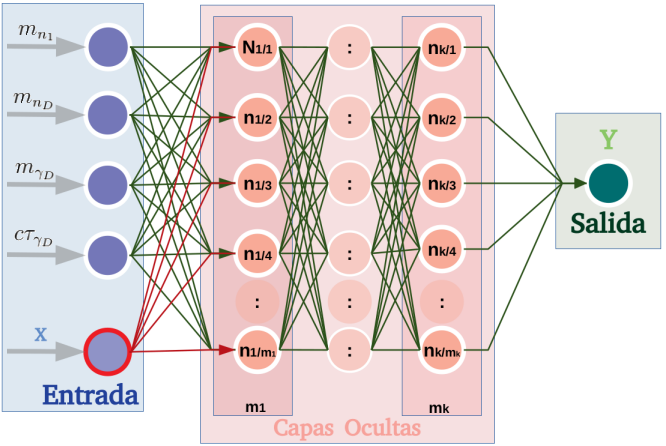
\includegraphics[width=.9\textwidth]{Cap3/imagenes/neuronas.png}
\caption{Diagrama de la estructura general de la red neuronal para regresión.}
\label{neuronas}
\end{figure}

%También se permite cambiar la dimensión de los datos de entrada para que estas coincidan con las necesidades requeridas, siempre considerando como mínimas entradas las condiciones iniciales de generación y una variable extra en el caso de que sea necesario.